\documentclass[12pt,a4paper]{article}
\usepackage[utf8]{inputenc}
\usepackage[sectionbib,round]{natbib} 
%\usepackage[german]{babel}
\usepackage[T1]{fontenc}
\usepackage[scaled]{luximono}
\usepackage{graphicx}
\usepackage[colorlinks,pdfpagelabels,pdfstartview = FitH,bookmarksopen =
true,bookmarksnumbered = true,linkcolor = internallink,urlcolor =
internallink, plainpages = false,hypertexnames = false,citecolor = black]
{hyperref}
\usepackage{listings}
\usepackage{framed}
\usepackage[numindex]{tocbibind}
\usepackage{makeidx}
\usepackage[hang,small,bf]{caption}
%\usepackage{lscape}
\usepackage{pdflscape}
\usepackage{ifpdf} % Unterscheidung zwischen pdflatex & latex
%hyperref soll als letztes Paket eingebunden werden:
\usepackage{hyperref} 

\ifpdf
\pdfinfo
{ /Title (ABL4J Developer Documentation)
  /Author (Stephan Schwiebert)
  /CreationDate (D:20091231201500) % this is the format used by pdf for
  /Subject (A developers guide to Alignment Based Learning for Java) 
  /Keywords (ABL, ABL4J)
}
\fi


\setcounter{secnumdepth}{4}
\setcounter{tocdepth}{4}

%TODO definieren:
% use index package to create indices
% \usepackage{index}
 % use color package to make todos jump out in text
 \usepackage{color}
 % start todo list
% \newindex{todo}{todo}{tnd}{Todo List} 
 % macro for todo entries addition
 \newcommand{\todo}[1]{\textcolor{red}{[To do: #1]}\index[todo]{#1}}

% Für inline-Code (vollqualifizierte Klassennamen o.ä.)
 \newcommand{\code}[1]{{\ttfamily\selectfont{#1}}}
 
 % Vereinfachung für Links, die komplett im Text abgedruckt werden sollen:
 \newcommand{\link}[1]{\href{#1}{#1}}

%\makeindex
\begin{document}

\title{Alignment Based Learning for Java -- A developers guide\thanks{Early
draft version for ABL4J 0.97}}
\author{Stephan Schwiebert}

\maketitle

\definecolor{internallink}{rgb}{0,0,1}


%\bibliographystyle{apalike}
\bibliographystyle{natdin}

%\renewcommand*{\dictumwidth}{.4\textwidth} 

\makeatletter

\makeatother

\renewcommand{\topfraction}{.8} 

\lstnewenvironment{java}[1][]
{\lstset{language=Java, 
		 morekeywords={enum},
		 basicstyle=\ttfamily\scriptsize,
		 xleftmargin=20pt,
		 xrightmargin=20pt,
		 breaklines=true,
		 breakatwhitespace=true,
		 frame=single,
		 float=htbp,
		 framexleftmargin=5pt,
		 framexrightmargin=5pt,
		 framextopmargin=5pt,
		 framexbottommargin=5pt,
		 captionpos=b,
		 #1
		}
} 
{}

\lstnewenvironment{cpp}[1][]
{\lstset{language=c, 
		 basicstyle=\ttfamily\scriptsize,
		 xleftmargin=20pt,
		 xrightmargin=20pt,
		 breaklines=true,
		 breakatwhitespace=true,
		 frame=single,
		 float=htbp,
		 framexleftmargin=5pt,
		 framexrightmargin=5pt,
		 framextopmargin=5pt,
		 framexbottommargin=5pt,
		 captionpos=b,
		 #1
		}
} 
{}

\lstnewenvironment{xml}[1][]
{\lstset{language=XML, 
		 morekeywords={enum},
		 basicstyle=\ttfamily\scriptsize,
		 xleftmargin=20pt,
		 xrightmargin=20pt,
		 breaklines=true,
		 breakatwhitespace=true,
		 frame=single,
		 float=htbp,
		 framexleftmargin=5pt,
		 framexrightmargin=5pt,
		 framextopmargin=5pt,
		 framexbottommargin=5pt,
		 captionpos=b,
		 #1
		}
} 
{}

%\tableofcontents
\abstract{
ABL4J is a Java port of Menno van Zaanen's Alignment Based Learning (ABL)
algorithm\footnote{see \link{http://ilk.uvt.nl/~menno/research/software/abl}}.
The idea of ABL4J was a) to make ABL available for Java developers and b) to
offer them a flexible alignment framework that can be extended in several ways.
As ABL is a popular alignment tool (if one can say that linguistic alignment
tools can be popular at all), I decided to use the codebase of ABL 1.1 for the
base functionality of ABL4J. This allows developers to compare their alignment
methods with ABL's methods, so one can easily see if a new algorithm is an
improvement or not.

This paper is structured as follows. Section \ref{usage} will explain how ABL4J
can be used within another Java application. In section \ref{customization}, the
architecture of ABL4J will be presented, thus demonstrating how new algorithms
can be added to the framework. Section \ref{configuration} will give an overview
of both existing options of ABL and new options introduced with ABL4J. Finally,
section \ref{junit} will explain how JUnit can be used with ABL4J to compare the
processing results of ABL and its Java port.}

\section{Introduction}
This paper is a developer's documentation to get familiar with the architecture
of ABL4J. Thus, it will not explain the theoretical concepts of ABL, or the
concrete implementations of ABL's algorithms. Instead, it is highly recommended to
read \cite{vanZaanen:2001p141} and \cite{vanZaanen:2003p72} for a description
of alignment in computational linguistics and \cite{Geertzen:2006p11} for a
description of the architecture and parameters of ABL first.

As the Eclipse IDE\footnote{\link{http://www.eclipse.org}} was used to develop
ABL4J, the project can be checked out from its SVN repository directly to an
Eclipse workspace. The project reexports all dependencies for both java
applications and Eclipse plugins, thus, it can simply be added to the project
dependencies of another project.

\section{Usage}
\label{usage}
To use ABL4J within a Java application, only a few lines of code are needed.
Assuming you added all required libraries to your project, this section shows
how align, cluster, and select are executed.

\begin{java} [caption={Programmatically configuring ABL4J},label={abl_code_configure}] 
		// Initialize ABL4J: ABLInitializer initializer = new ABLInitializer();
		Properties props = new Properties();
		props.put(AblProperties.INPUT_FILE, "testdata/input/input.txt");
		props.put(AblProperties.OUTPUT_FILE, "testdata/output.txt");
		initializer.initialize(null, props);
		PropertiesMap properties = initializer.getProperties();
		
		// Create a new Treebank
		ITreeBank treeBank = DataFactory.newTreeBank();
		ITreeBankReader reader = IOFactory.getReader(properties);
		reader.readTreebank(treeBank);
\end{java}

As Listing \ref{abl_code_configure} shows, the \emph{PropertiesMap} is a very
important part of ABL4J, as it defines which data is processed, and how the
processing within align, cluster or select is further specified. Here,
most options are defined non-programmatically to keep the example simple.
However, section \ref{configuration} gives a detailed overview of all
build-in configuration options and section \ref{customization} shows how custom
algorithms can be implemented and added to the framework. Once ABL4J has been
set up, a treebank can be created and filled with data to be analyzed, as shown
in Listing \ref{abl_code_new_tb}. Note that the treebank returned from the
factory is an interface -- this allows to use different treebank
implementations without modifying any code.

\begin{java} [caption={Creating a new Treebank},
label={abl_code_new_tb}] 
		// Create a new Treebank
		ITreeBank treeBank = DataFactory.newTreeBank();
		ITreeBankReader reader = IOFactory.getReader(properties);
		reader.readTreebank(treeBank);
\end{java}

The reader which is used to read a treebank is also returned by a factory method, thus one
can implement a custom reader for any new treebank format and simply configure
the framework to use this reader. For example, ABL4J comes with a treebank reader
for the Tiger Corpus\footnote{see
\link{http://www.ims.uni-stuttgart.de/projekte/TIGER/TIGERCorpus/} for details}
format, which converts the manually created annotations within that corpus to ABL
compatible data structures. A treebank reader for the British National Corpus
will be added soon.

To process the data loaded into the treebank, instances of Align, Cluster and
Select have to be created, configured and executed. Listing \ref{abl_code_exec}
show how this can be done.

\begin{java} [caption={Running ABL Components}, label={abl_code_exec}] 
		// Create, configure and execute Align, Cluster, and Select components
		Align align = new Align();
		Cluster cluster = new Cluster();
		Select select = new Select();
		align.configure(properties);
		cluster.configure(properties);
		select.configure(properties);
		
		// Execute components
		align.execute(treeBank);
		cluster.execute(treeBank);
		select.execute(treeBank);
\end{java}

Finally, the processed data should be stored somewhere, so in listing
\ref{abl_code_store} the IOFactory is asked for a writer to store the treebank.

\begin{java} [caption={Storing the new Treebank}, label={abl_code_store}] 
		// Write treebank
		ITreebankWriter writer = IOFactory.getWriter(properties);
		writer.writeTreebank(treeBank);
\end{java}

Note that in listing \ref{abl_code_new_tb} and \ref{abl_code_store} no file
names are used -- this information is contained within the PropertiesMap given
to the factory. This might be a bit confusing, as the IO-code does not
show which files are processed, but on the other hand one can freely connect
ABL4J to any storage system, in which, for example, custom readers and writers
use custom properties to load and store treebanks within a database, use data
already contained in memory, or something similar.

The complete listing can be found in class \code{Example1}. If executed, some
Log4J-Messages should be printed and the results of the alignment should be
found in file \emph{testdata/output.txt}.


\section{Customization}\label{customization}
Most parts of ABL4J make intensive use of Java interfaces and thus offer
several ways to add new functionality. In general, all these interfaces are
related to one of the following:

\begin{itemize}
  \item Internal data structures, like the implementation of ITreebank or
  IConstituent,
  \item IO-operations to serialize and deserialize treebanks, or
  \item Algorithms that perform the align, cluster, or select step of ABL.
\end{itemize}

The rest of this section will give a basic overview of these parts of ABL4J.

\subsection{Data Structures}

If the implemented data structures do not fit the requirements of a new
algorithm, or if the architecture of an application that uses ABL4J needs a
different implementation, the interfaces found in package
\code{org.schwiebert.abl4j.data} can be reimplemented. Figure \ref{data_img}
shows a class diagram of these interfaces. 

\begin{figure}
  \centering
  \fbox{
    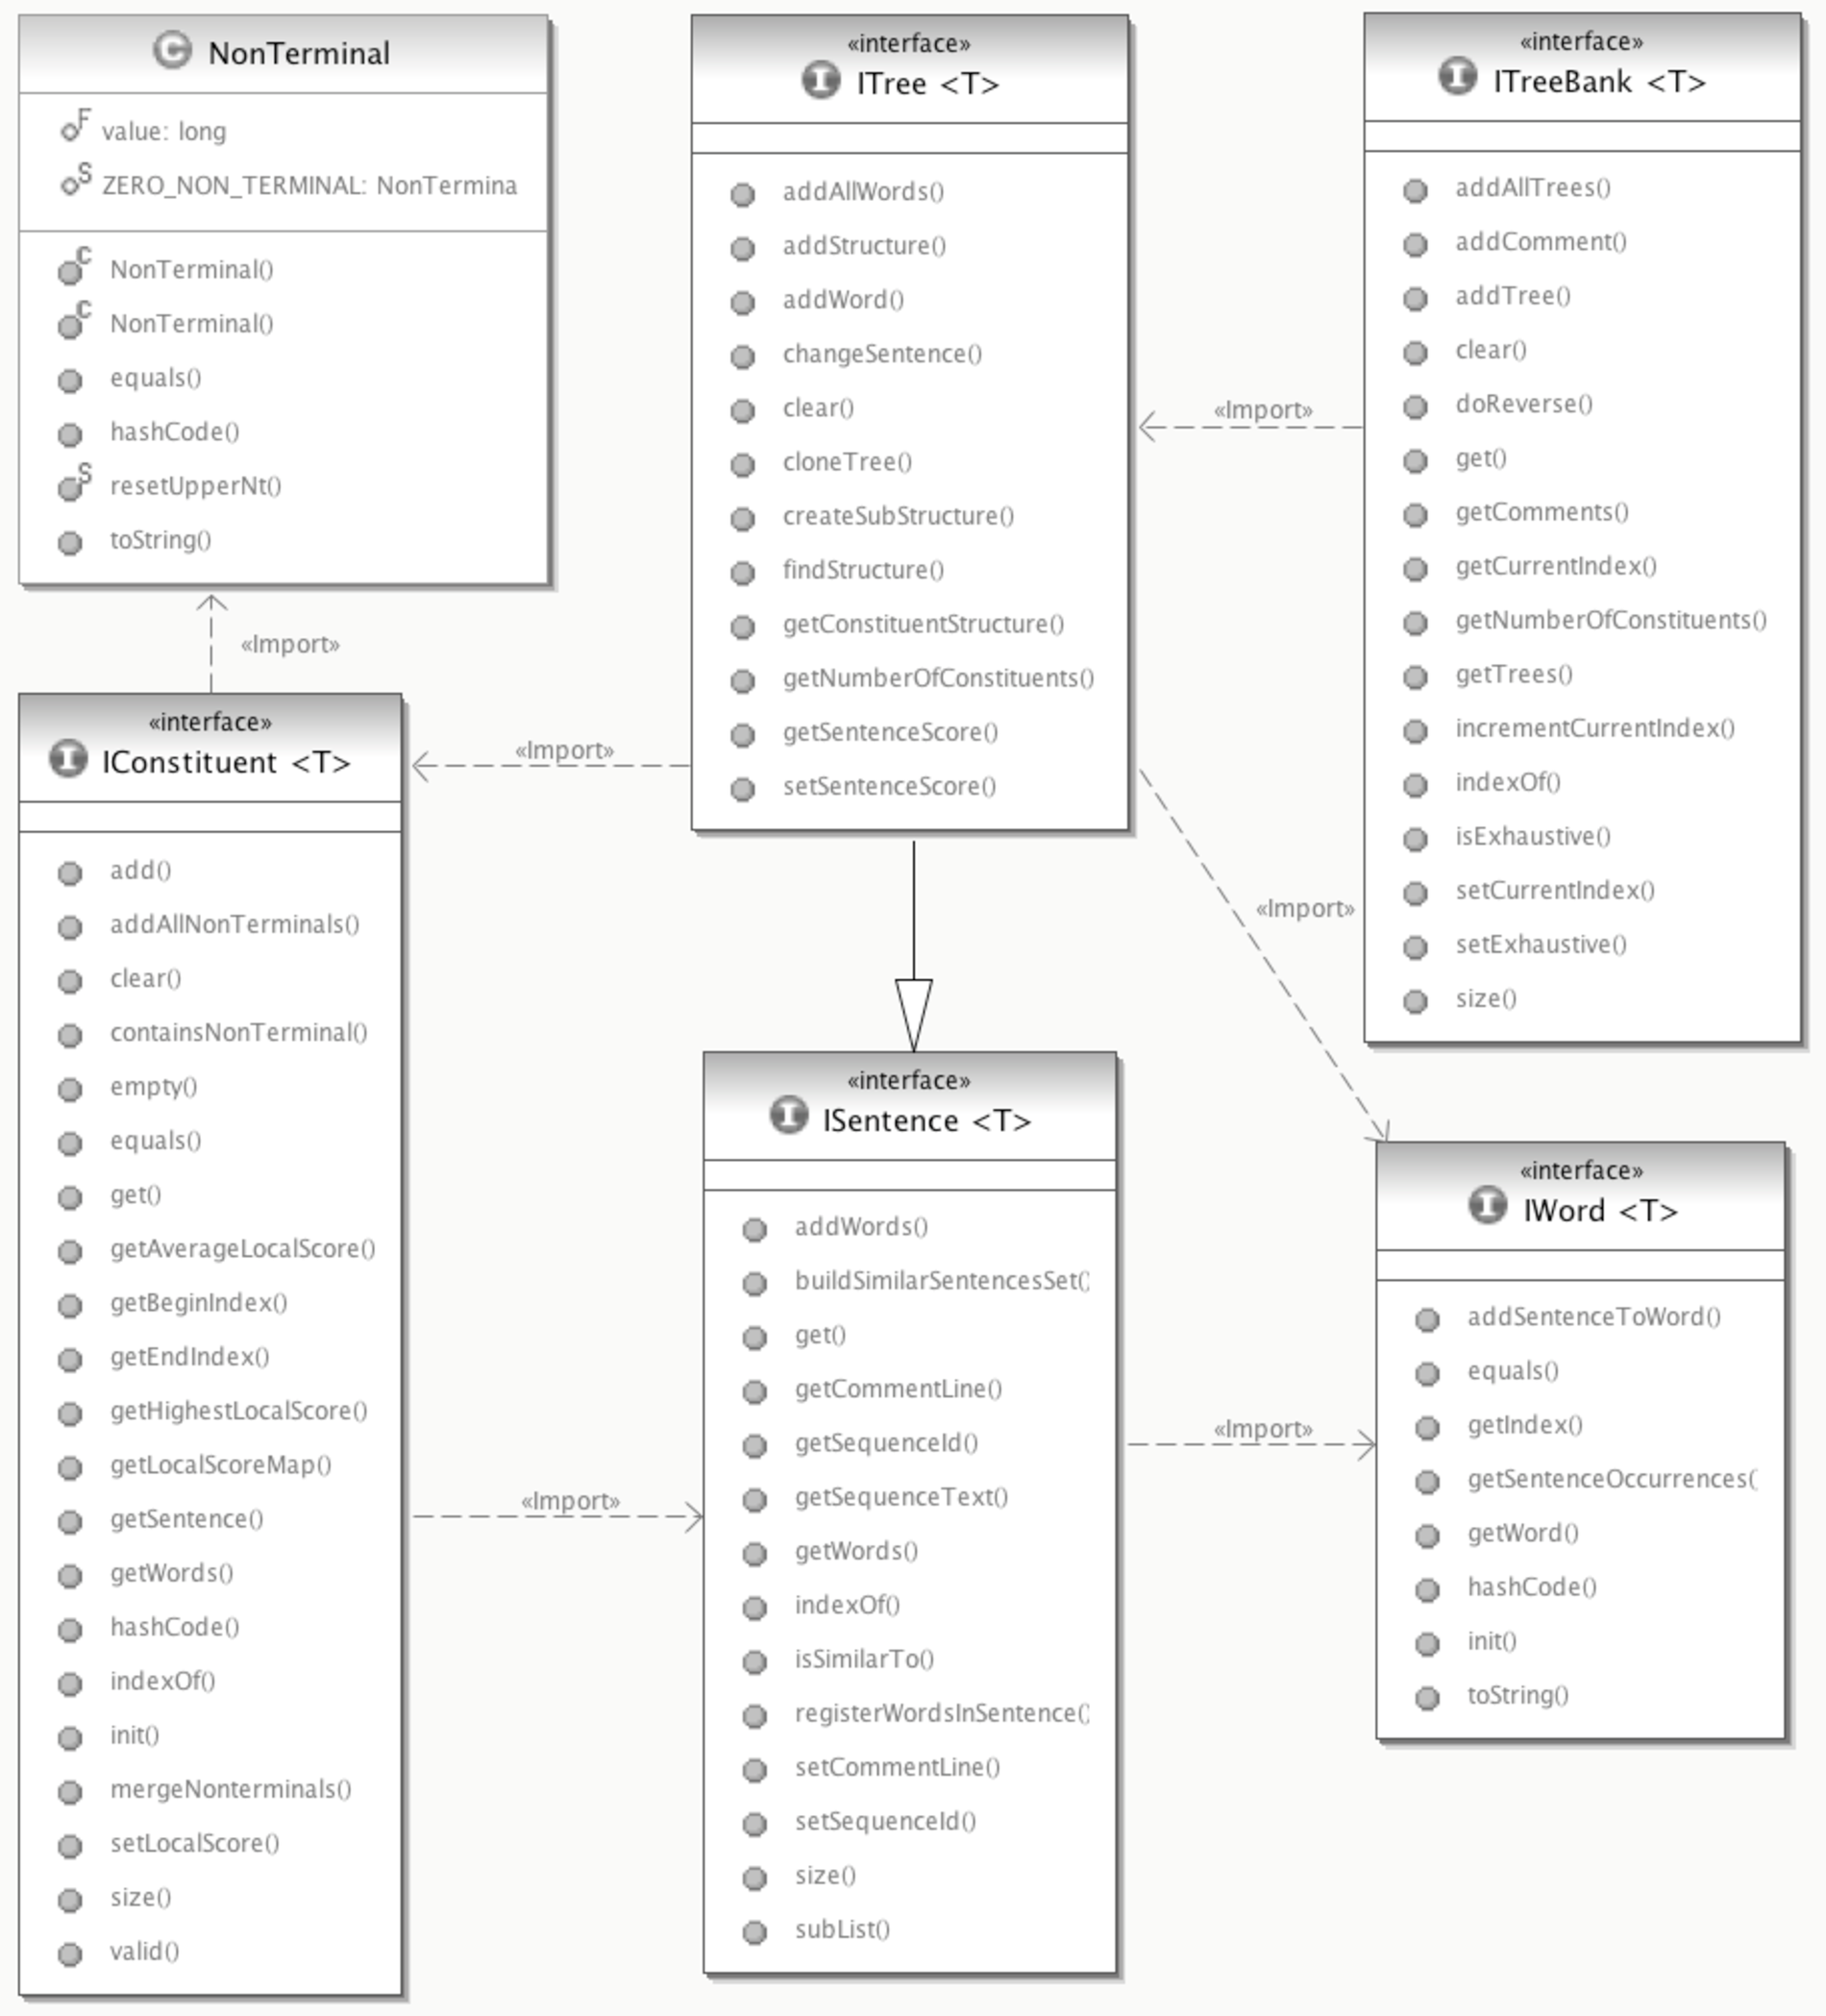
\includegraphics[width=1\textwidth]{data}
  }
  \caption{Internal Data Structures}
  \label{data_img} 
\end{figure} 

To make use of the new classes, the corresponding properties (see table
\ref{additional_options}) must be set to the fully qualified class name of the
custom classes. Additionally, the mapping of terminal symbols can be modified.
ABL originally maps words (strings) to integers and makes a reference to these in
its data structures, however, if another kind of data shall be aligned, a new
\code{IWordMapping} can be implemented. In most cases, only a new
\code{java.util.Comparator} has to be passed to the constructor of the default
implementation \code{WordMapping}, as shown in Listing \ref{stringmapping} for
the default word mapping implemented for strings. As with data structures, the
word mapping must be set by the corresponding property (see table
\ref{additional_options}).

\begin{java} [caption={Constructor of class StringMapping},label={stringmapping}] 
	public StringMapping() { 
		super(new Comparator<String>() {
			public int compare(final String o1, final String o2) {
				return o1.compareTo(o2);
			}
		});
	}
\end{java}

\subsection{IO}

As listings \ref{abl_code_new_tb} and \ref{abl_code_store} showed,
IO-operations are encapsuled in \code{ITreebankReader} and
\code{ITreebankWriter}. To support new data formats, one can either implement
these interfaces (or one of them to support a custom format as input or output only,
as in case of the \code{TigerCorpusReader}), or extend one of the existing
implementations. Figure \ref{io_img} gives an overview of the IO-related
classes and interfaces which are currently available in ABL4J. 

\begin{figure}
  \centering
  \fbox{
    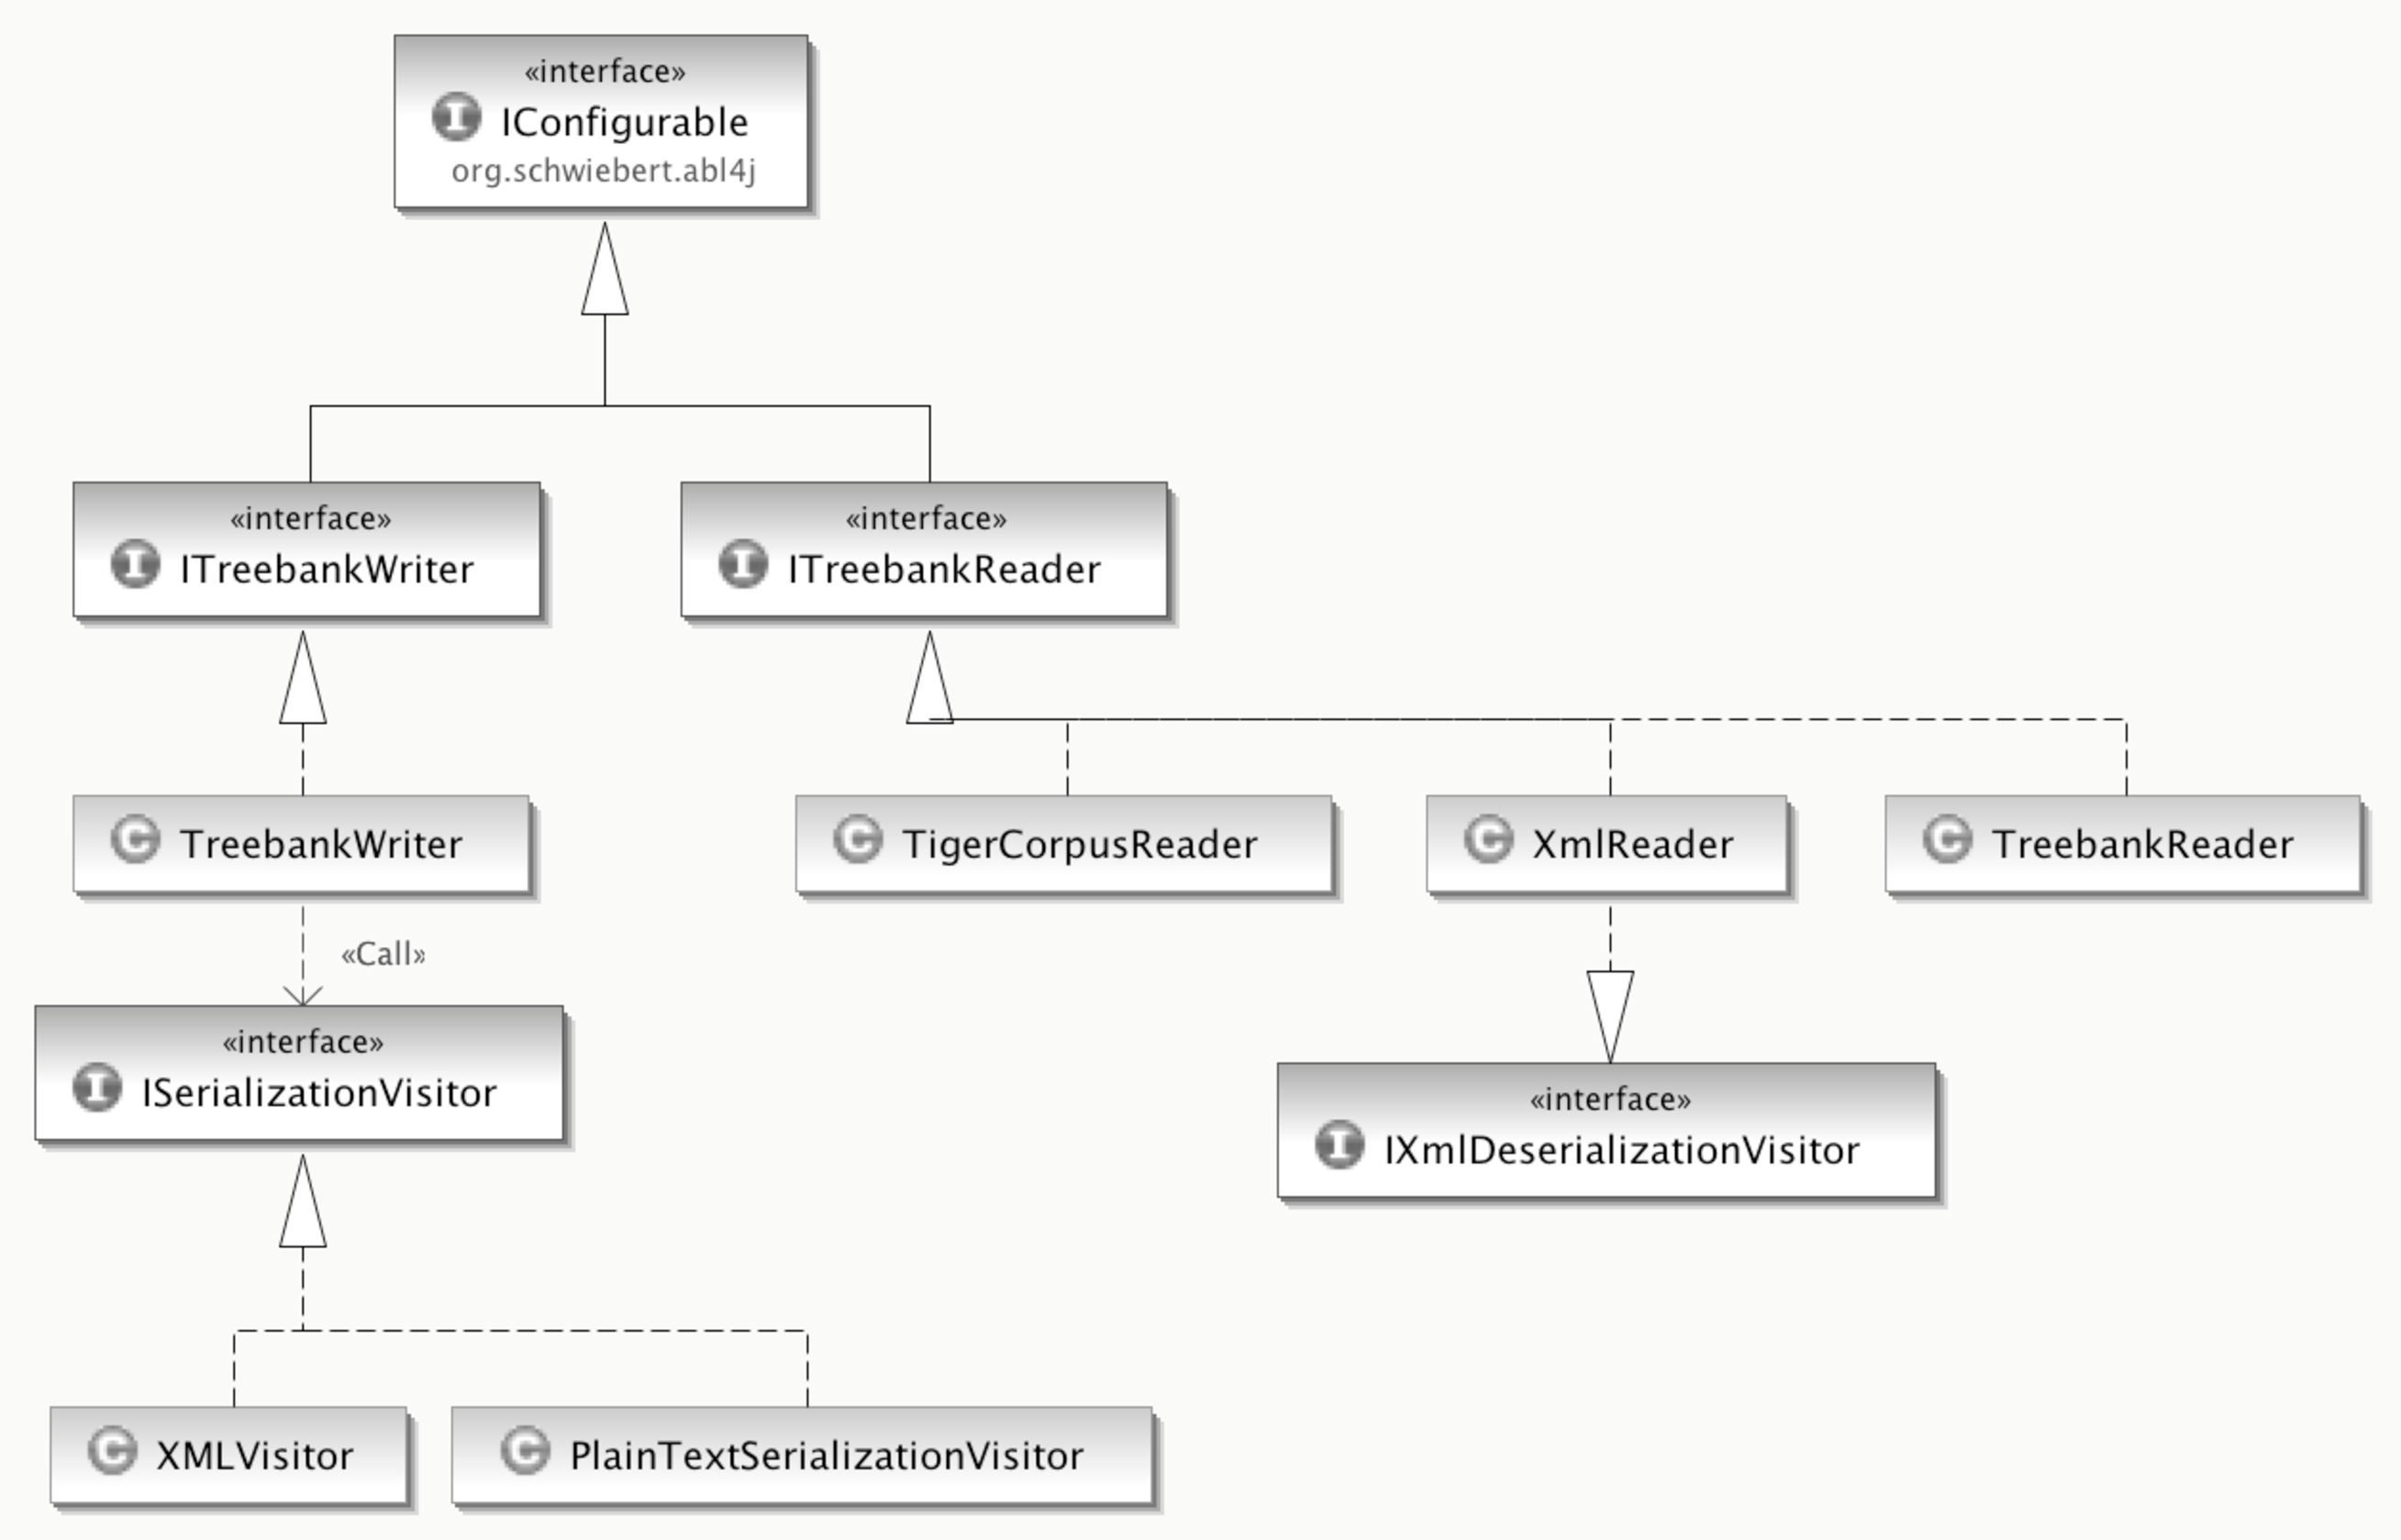
\includegraphics[width=1\textwidth]{io}
  }
  \caption{IO-System in ABL4J}
  \label{io_img} 
\end{figure} 

Additionally, a
\emph{visitor}-pattern has been integrated in ABL4J, so that serialization
and deserialization can be further simplified: If, for instance, a new data
format should be written, the \code{ISerializationVisitor}-interface can be
reimplemented and set for use within the default serializer via the
\code{serialization.visitor} property (see section \ref{custom_properties}).
Thus, no code for visiting the treebank data structure must be implemented.
However, as the visitor pattern requires that the structure of the visited
data is known, a deserialization visitor is available only for deserializing
XML formats.

Note that ABL4J does not define the kind of data source or destination --
instead, readers and writers can be implemented to use files, streams, or something similar.
The existing readers and writers support files and streams by using the
properties \code{input.file} or \code{input.stream} for reading and
\code{output.file} or \code{output.stream} for writing. If none of these
properties is set, the default streams \code{System.in} and \code{System.out} are
used. In this case, the streams won't be closed after serialization or
deserialization.

\subsection{Algorithms}
Customization of data structures and IO functionality is probably
required only to integrate ABL4J into another architecture. To modify the
produced structures, or to test new hypotheses, new algorithms can be added to
ABL4J by implementing one of the interfaces \code{AlignmentMethod},
\code{ClusterMethod}, or \code{SelectMethod}. Figure \ref{align_methods} gives
an overview of the existing alignment methods of ABL, and how they are
integrated into ABL4J.


\begin{figure}
  \centering
  \fbox{
    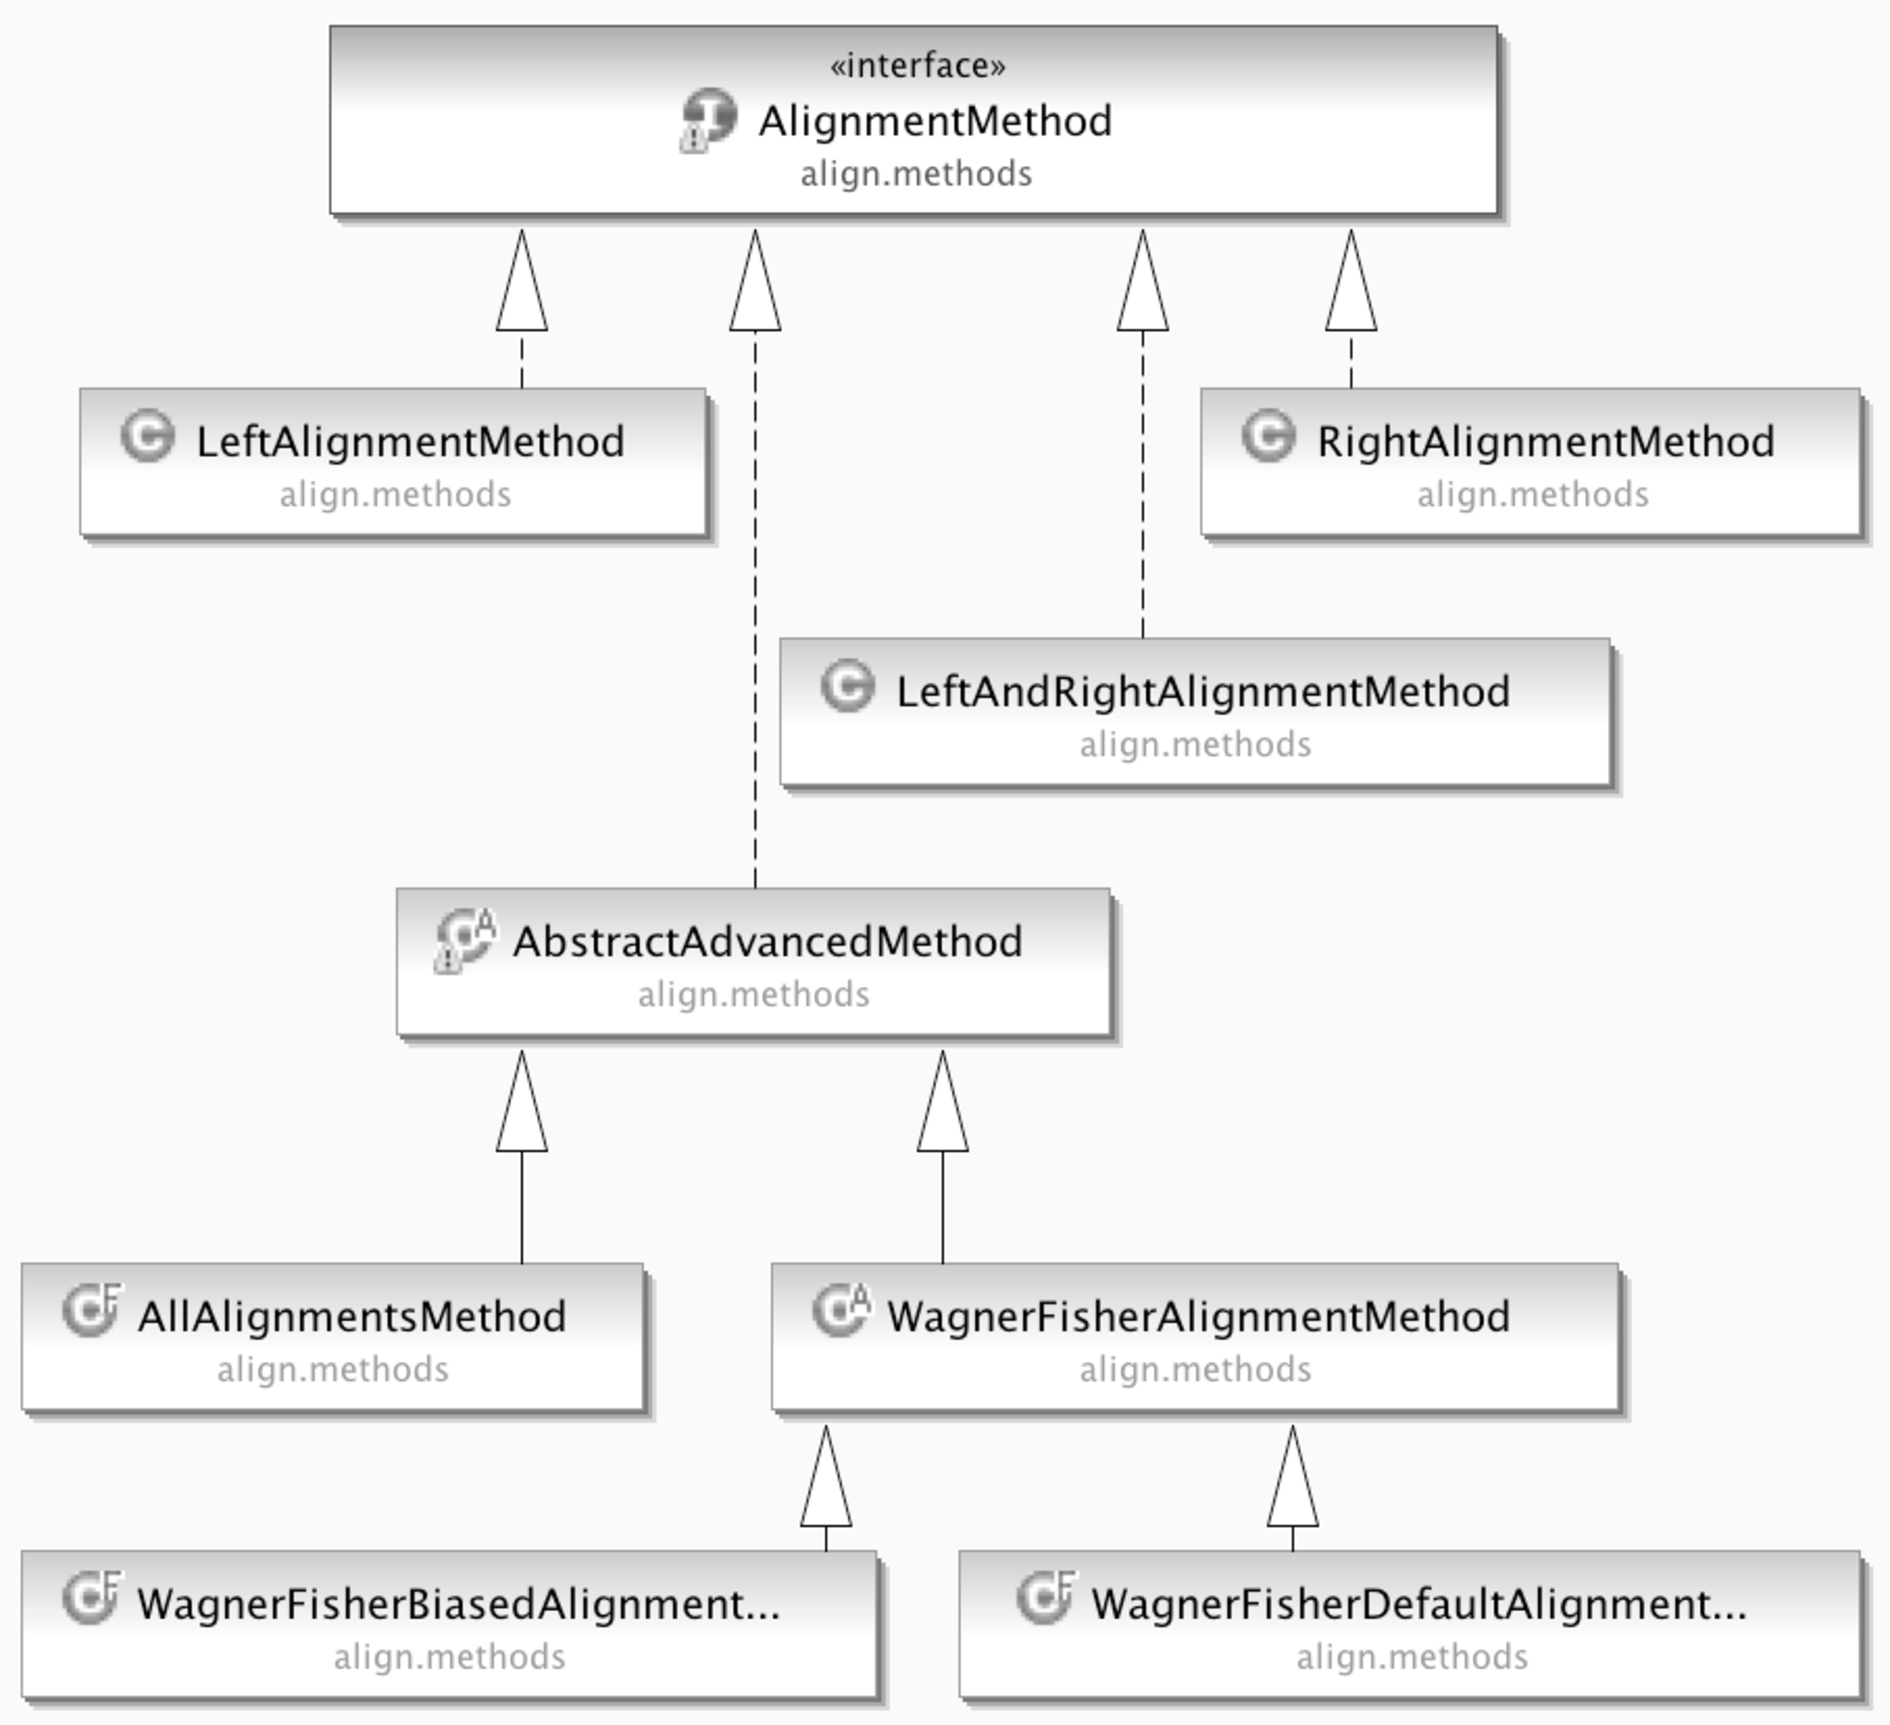
\includegraphics[width=1\textwidth]{align_methods}
  }
  \caption{Hierarchy of implemented alignment methods}
  \label{align_methods} 
\end{figure} 

In general, an alignment method compares tree structures and generates
constituent hypotheses. A clustering method groups these hypotheses, and a
select method detects and removes incompatibilities between hypotheses -- see
\cite{vanZaanen:2003p72} for a detailed description of these ideas.

\section{Configuration}\label{configuration}
The original ABL programs \emph{align}, \emph{cluster} and \emph{select} can be
configured by several command line options. Most of these options can be used to
launch the ABL4J ports of these programs, however, some of them are not
supported (as, for instance, ABL4J uses Log4J for logging, so no custom log
architecture was implemented). Also, if ABL4J is used within another Java
application, other ways of configuring parameters are needed. This section
describes the way ABL4J can be configured.

\begin{landscape}
\begin{figure}[htb]
  \centering
  \fbox{
    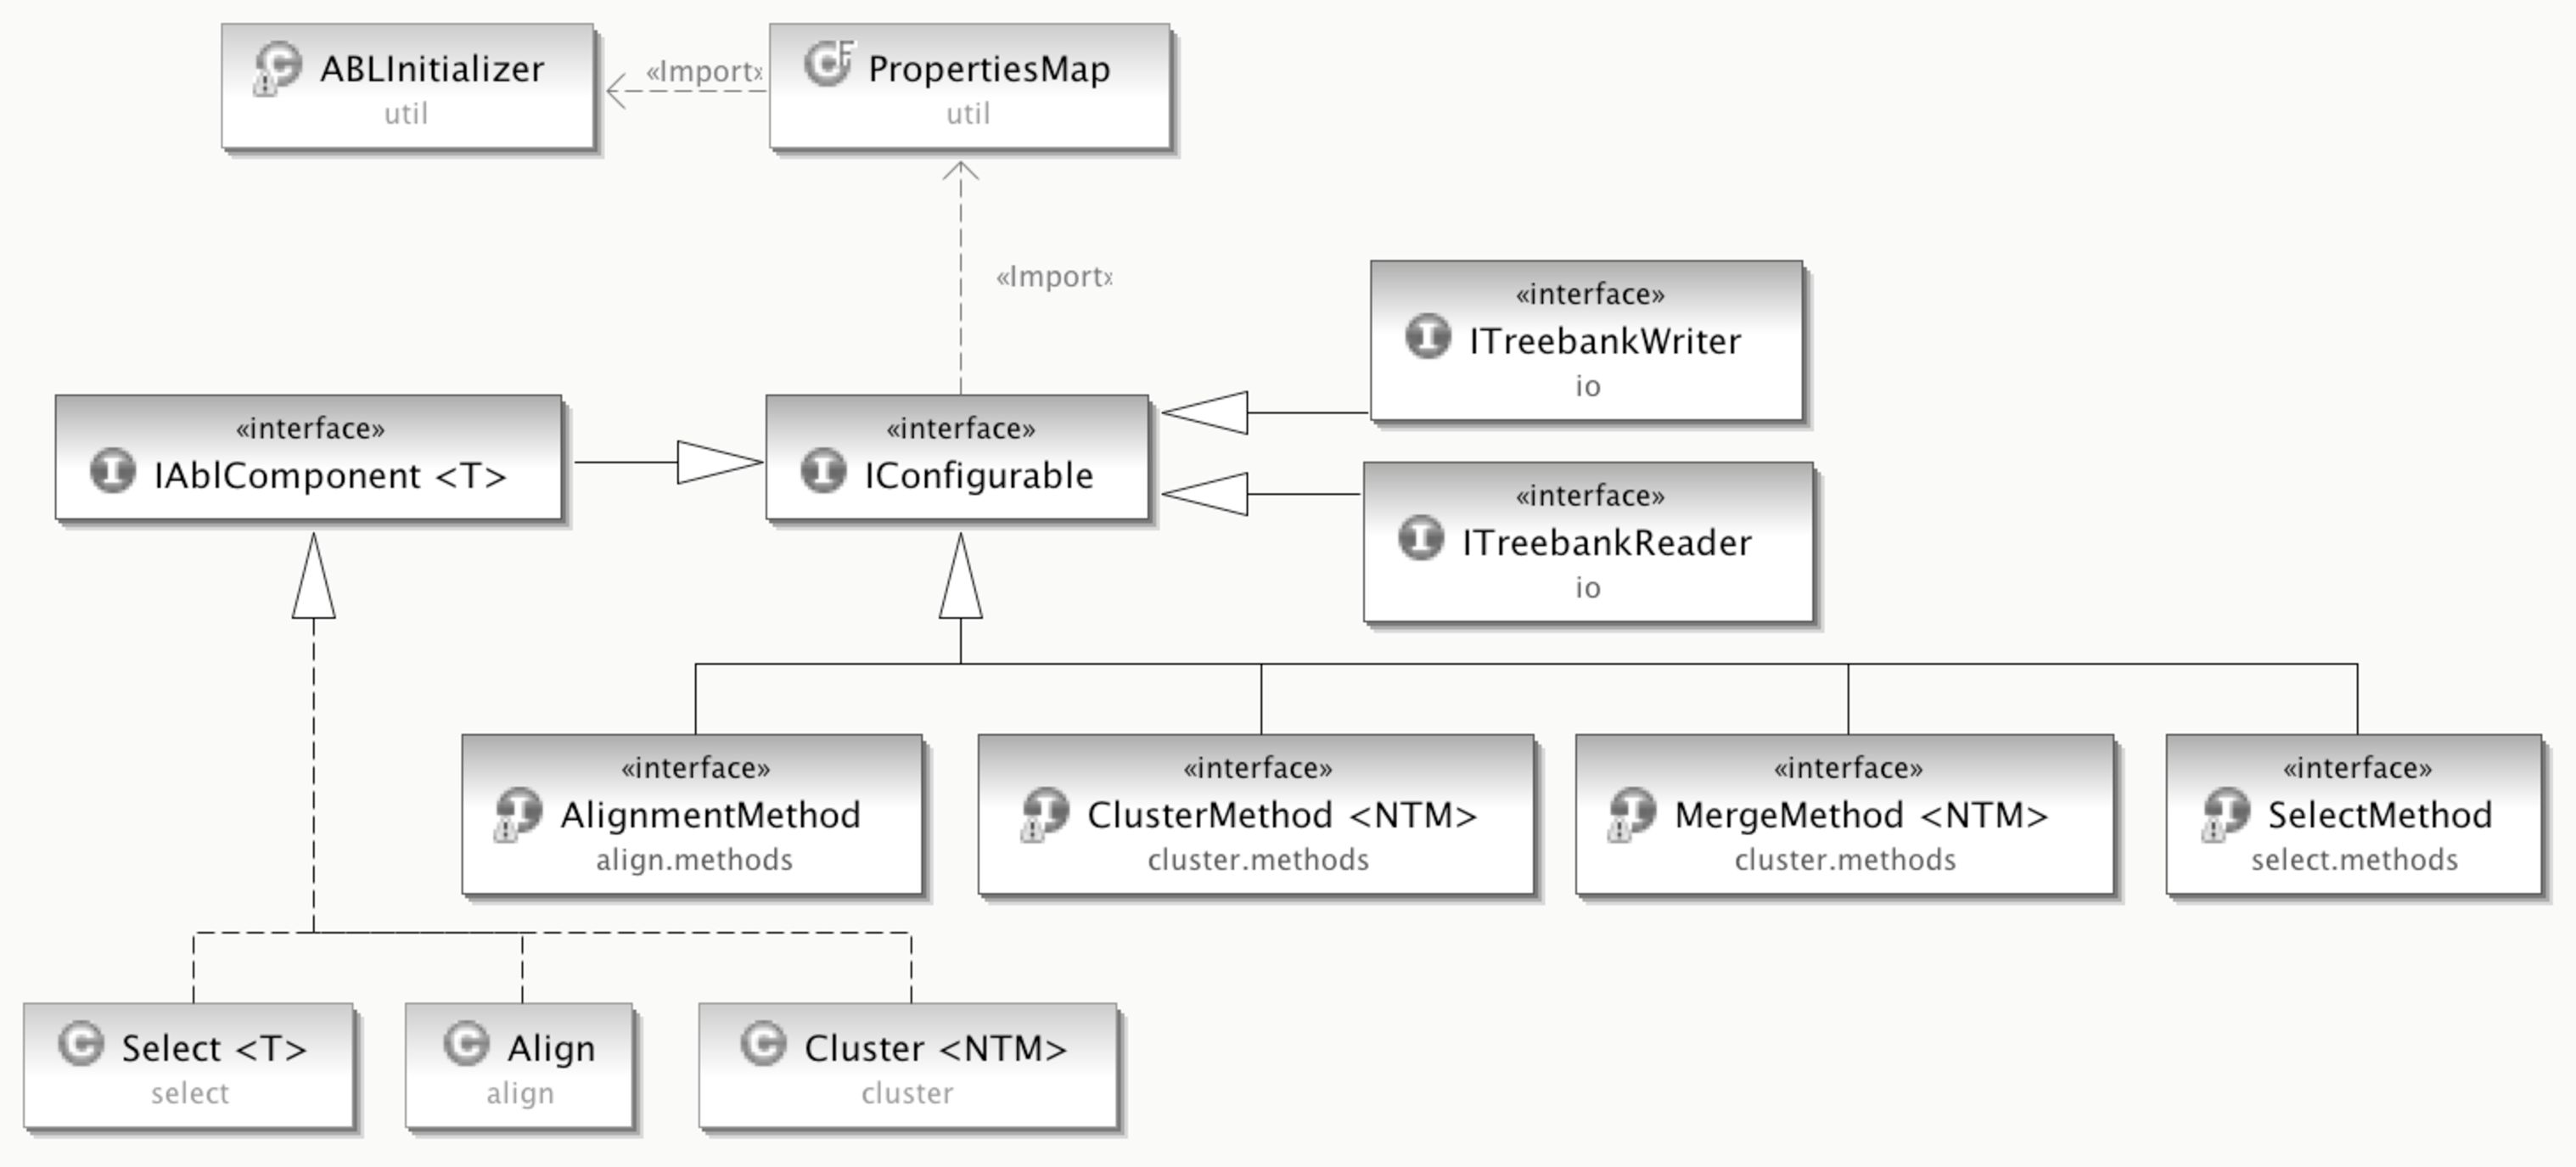
\includegraphics[width=1.6\textwidth]{init}
  }
  \caption{Overview of configurable elements in ABL4J}
  \label{init_img} 
\end{figure} 
\end{landscape}

\subsection{Configuration sequence}

Before one of the classes \code{Align}, \code{Cluster}, or \code{Select} can be
used, it must first be configured by calling \code{configure(PropertiesMap map)}.
This method starts the configuration process, which is based on Java's properties
system. First, some properties will be set to default values to simplify the
required configuration -- see tables \ref{abl_cmd_line} and
\ref{custom_properties} for details. Than, ABL4J will search for a file called
\emph{abl4j.properties} on the classpath. If found, the properties defined there
will be added to the set of properties, probably overriding any default values
set before. Finally, if ABL4J is launched from a command line, any options
defined there will be added to the properties map (again overriding already
defined properties with the same name). If ABL4 is integrated in another java
application, this step will be skipped -- instead, properties can be set
programmatically by calling \code{PropertiesMap.put(String key, String value)}
before an ABL4J component is initialized (see section \ref{usage}).

% etc.
\begin{landscape}


\begin{table}
\label{abl_cmd_line}

\begin{tabular}[h]{|p{3.2cm}|p{1.5cm}|p{3.5cm}|p{3cm}|p{3cm}|p{3.2cm}|p{2.5cm}|}
\hline 
Name & ABL option & ABL4J property & Supported values & ABL4J values & Default
value & Component\\ \hline Input File & -i & input.file & any filename &
any filename & null (System.in) & all\\ \hline 
Output File & -o & output.file & any filename & any filename & null
(System.out) &all\\ \hline Align type & -a &
align.method & a, l, r, b, aa, wm, wb (but not st1\ldots st4) & fully qualified
class name & \ldots align.methods.\newline AllAlignment & align\\ \hline Part
type & -p & part.type & e, u, b & enum PartType & unequal &align\\ \hline Exclude Empty & -e &
align.exclude.empty & -- & boolean &false &align\\ \hline No Merge & -n &
align.nomerge & -- & boolean &false &align\\ \hline Exhaustive & -x &
align.exhaustive & -- & boolean &false &align\\ \hline Select Type & -s
&select.type & f, t, c, b &enum SelectType &\ldots
select.methods.\newline ConstituentSelect\newline Method &select\\ \hline Seed
& ?? &seed & integer & integer &0 &align, select\\ \hline Verbose & -v & not supported & -- & -- &false & all\\ \hline Preserve& -m &select.preserve & -- &
boolean & false &select\\ \hline

\end{tabular}
\caption{ABL options and their ABL4J equivalents. Note: All ABL4J properties
and fully qualified class names begin with the prefix
\emph{org.schwiebert.abl4j.}}
\end{table}
\end{landscape}


As ABL4J uses Log4J for logging, ABLs logging flags are not supported. Instead,
logging can be configured by modifying file \emph{log4j.properties} found in
the project's root directory\footnote{If you are not familiar with Log4J, visit
\link{http://logging.apache.org/log4j/}.}.

\subsection{ABL4J properties}\label{custom_properties}
ABL4J adds several options to the set of options used by ABL. Most of these are
architecturally required and cannot be defined via command line, as they are
intented to be used only in applications that use ABL4J as a library. Table
\ref{additional_options} gives an overview of these options.
The options \emph{compatibility.mode} is used for debugging, in particular to
compare the results of ABL and ABL4J. This is the only option that can be used
from command line by adding the parameter \emph{-j}. See section \ref{junit}
for further details. As parts of ABL4J support multithreading, the number of
threads can be defined by setting \emph{threads} to an integer greater than 1
-- see section \ref{multithreading}. If \emph{reset.upper.nt} is set to
\code{true}, during initialization of align, cluster, or select, the largest
unused non terminal id is set to 0. The options \emph{cluster.method} and
\emph{merge.method} can be used to partially modify the clustering phase of ABL
instead of implementing a new cluster method.

\begin{landscape}
\begin{table}
\label{additional_options}
\begin{tabular}[h]{|p{4cm}|p{3.5cm}|p{5.0cm}|p{5.5cm}|p{2cm}|} \hline
Name & Property & Supported values & Default value & Component \\ \hline
Compatibility Mode &compatibility.mode&boolean&false&all\\ \hline
Reader Class&reader.class&fully qualified class name&\ldots
io.TreebankReader&all \\ \hline Writer Class&writer.class&fully qualified class
name&\ldots io.TreebankWriter&all \\ \hline Serialization
Visitor&serialization.visitor&fully qualified class name&\ldots
io.\newline PlainTextSerializationVisitor&all \\ \hline Cluster
Method&cluster.method&fully qualified class name&\ldots cluster.methods.\newline ABLClusterMethod&cluster \\ \hline Merge
Method&merge.method&fully qualified class name&\ldots
cluster.method.\newline ABLClusterMethod&cluster \\ \hline Input
Encoding&input.encoding&String&UTF-8&all \\ \hline Output Encoding&output.encoding&String&UTF-8&all \\ \hline Number of
Threads&threads&integer&1&align \\ \hline Comparism
Mode&comparism.mode&boolean&false&all \\ \hline Constituent Class
&constituent&fully qualified class name&\ldots data.Constituent&all\\ \hline
Sentence Class&sentence&fully qualified class name&\ldots data.Sentence&all \\
\hline Treebank Class&treebank&fully qualified class name&\ldots
data.Treebank&all \\ \hline Word Class&word&fully qualified class name&\ldots
data.Word&all \\ \hline Tree Class&tree&fully qualified class name&\ldots data.Tree&all \\ \hline Reset Upper
NT&reset.upper.nt&boolean&true&all \\ \hline Word Mapping&word.mapping&fully
qualified class name&\ldots util.StringMapping&all\\ \hline
Input Stream&input.stream&instance of java.io.InputStream&
null&all\\ \hline
Output Stream&output.stream&instance of java.io.OutputStream&
null&all
\\
\hline

\end{tabular}
\caption{Additional ABL4J properties. Note: All ABL4J properties and fully
qualified class names begin with the prefix \emph{org.schwiebert.abl4j.}}
\end{table}
\end{landscape}

\section{Multithreading}\label{multithreading}
In general, it is possible to execute multiple instances of ABL4J within the
same virtual machine, even with different parameters. However, as this feature
has not been tested well yet, it is still experimental and might cause problems.
\\
Besides that, the align and select phases of a single instance of ABL4J can be
run in several threads, thus improving the overall performance on multi core
or multi processor pc's. However, to support this feature, it is important that
new algorithms or data structures do not use \emph{static} fields, as this
would probably lead to unexpected results. Instead use, for instance,
\code{java.lang.InheritableThreadLocal} to create "`pseudo-static"' variables.



\section{JUnit -- comparing ABL and ABL4J}
\label{junit}
While porting ABL to Java, a JUnit Test Suite was used to compare the treebanks
produced by ABL and ABL4J. The goal was to produce exactly the same structures
that were produced by ABL, as this is what one expects if using a ported
framework. However, there were a few differences between Java and C++ that
required modifications of both ABL4J and ABL. So, if you want to ensure that
ABL4J does work as expected, you will unfortunately have to do some work first.
Otherwise you can skip this section.

ABL4J can be used with a \emph{compatibility flag} that forces the program to
produce exactly the same output as the C++ version. For instance, if it is set
to \code{true}, all random numbers are generated by calling a native C
function, so random based parts (like the \emph{both} alignment method or
the select component) execute equally. However, another difference between C
and Java is related to rounding double-values, and as a workaround the related 
functions of ABL were modified. So, in order to compare the data produced by ABL
and ABL4J, a few changes must be made to the ABL source code, as shown in
\ref{align_cpp} and \ref{select_cpp}.

\begin{cpp} [caption={Required Changes in Align.cpp},
label={align_cpp}] 

Replace

Sub_dis(Ran b1, Ran e1, Ran b2, Ran e2) throw() 
     :Sub<Ran>(b1, e1, b2, e2) {
      for(; b1!=e1;b1++) { len1++; }
      for(; b2!=e2;b2++) { len2++; }
   };

with

Sub_dis(Ran b1, Ran e1, Ran b2, Ran e2) throw() 
     :Sub<Ran>(b1, e1, b2, e2) {
	len1 = 0; len2 = 0;
      for(; b1!=e1;b1++) { len1++; }
      for(; b2!=e2;b2++) { len2++; }
   };
\end{cpp}


\begin{cpp} [caption={Required Changes in Select.cpp},
label={select_cpp}] 
Insert the following two functions

bool isLess(double a, double b) {
	double result = a - b;
	result += 0.000001;
	return result < 0;
}

bool isLessOrEqual(double a, double b) {
	double result = a - b;
	if (result + 0.000001 < 0) {
		return true;
	}
	if(result < 0.000001) {
		return true;
	}
	return false;
}

and replace the tests
 
 ...
 if (((new_p=compute_combined_probability(t, res, prob))<=best_p) ||(uninit)) {
 ... if ((new_p>=0)&&(new_p<best_p)) {
 ...
     }
 }

 in select_prob_in_range with

...
 new_p = compute_combined_probability(t, res, prob);
 if (isLessOrEqual(new_p, best_p) ||(uninit)) {
 ...
 	if ((new_p>=0)&&(isLess(new_p, best_p))) {
 	...
 	}
 	...
 }
\end{cpp}

Finally, the native random code used by ABL4J in compatibility mode must be
compiled -- the source and header files can be found in dirctory \emph{c\_src}
of ABL4J. The compiled library than must be added to the java.library.path, which
can be done by placing it directly in the project root directory.
\\
Note that all these modifications are optional, as long as you do not expect
that ABL4J will produce \emph{exactly} the same results as ABL. However, if you
want to compare both versions and successfully compiled all required C++-code,
you can place the generated executables of align, cluster and select in the
directory \emph{orig} of the ABL4J project and then run the JUnit tests (in
correct order: align, cluster, select) found in the package
org.schwiebert.abl4j.tests. These tests will use the content of file
\emph{testdata/input/input.txt}, call both C++ and Java versions of the
program with every parameter variant and compare the processing results. They will fail if the results differ.
 
\section{Licence}
ABL4J is licensed unter the GNU Lesser General Public License (LGPL). Thus, it
can be used in any other software project without further license requirements.
However, if you add new features to it (as, for instance, new algorithms or
support of new data formats), it would be great if you would allow me to add
them to the library, so that other developers can benefit from them.

\newpage
\bibliography{UserDocumentation}

\end{document}
\endinput